\documentclass[12pt,a4paper,twoside,italian]{book} %twoside,
\raggedbottom % per evitare eccessivi spazi bianchi verticali

% Usare "oneside" invece di "twoside"
% nelle bozze, per risparmiare carta:
% "twoside" produce diverse pagine bianche
% alla fine dei capitoli.

\usepackage[utf8]{inputenc}
\usepackage[italian]{babel}
\usepackage[T1]{fontenc}
\usepackage{siunitx}

%interlinea 1.5
\linespread{1.5}

   %%%%%%%%%%%%%%%%%%%%%%%%%%%%%%%%%%%%%%%%%%%%%%%%%%%%%%%%%%%%
   % Se nella tesi si inseriscono dei passi in un'altra       %
   % lingua (inglese, per fissare le idee), si puo' istruire  %
   % il TeX di sillabare quella parte di testo con le regole  %
   % inglesi, invece che italiane. A questo scopo basta       %
   % scrivere                                                 %
   %                                                          %
   %    \documentclass[...,english,italian,...]{...}          %
   %                                                          %
   % al posto di \documentclass[...,italian,...],             %
   % dopodiche' la sillabazione sara' italiana fintanto che   %
   % non si incontra il comando \selectlanguage{english}.     %
   % Per tornare all'italiano si scrive                       %
   % \selectlanguage{italian}                                 %
   %%%%%%%%%%%%%%%%%%%%%%%%%%%%%%%%%%%%%%%%%%%%%%%%%%%%%%%%%%%%

% per la definizione dello stile di pagina e delle macro con le quali ridisegnare la pagina principale.
\usepackage{unisanniotesi}

% questo package è utilizzao per permettere l'utilizzo dell'ambiente algoritmic che consente di editare e formattare opportunamente frammenti di pseudocodice.
\usepackage{algorithmic}

%\usepackage{algorithm}  %algorithm serve per incapsulare algorithmic al fine di ottenere un oggetto flotable come una figura o una tabella.

% Col pacchetto tocbibind compariranno nell'indice anche
% la bibliografia ed eventualmente l'indice analitico
\usepackage[nottoc]{tocbibind}

% \usepackage{graphicx} % gia' caricato da unisanniotesi
\graphicspath{{./figure/}}
\usepackage{epstopdf}

% Per l'ipertesto:
% \usepackage{hyperref} % gia' caricato da unisanniotesi
\hypersetup{
  % pdfpagelayout=SinglePage, % default
  % pdfpagemode=UseOutlines, % default
  % bookmarksopen, % default
  % bookmarksopenlevel=2, % default;
  pdftitle={Fusione di dati Stereo e Time-of-Flight mediante tecniche di Deep Learning},
  pdfauthor={Francesco Pham},
  pdfsubject={Tesi sulla fusione di dati 3d da telecamere stereo e sensori Time-of-Flight mediante tecniche di Deep Learning},
  pdfkeywords={tesi laurea fusione 3d stereo time of flight deep learning}} 
%%%%%%%%%%%%%%%%%%%%%%%%%%%%%%%%%%%%%%%%%%%%%%%%%%%%%%%%%%%%

\usepackage{amsmath, amsfonts, amssymb, amsthm}
\usepackage{latexsym}

% altri pacchetti
\usepackage{float}
\usepackage{xcolor}
\usepackage{emptypage} % per nascondere la numerazione nelle pagine bianche
\usepackage{url}

\makeatletter
\renewcommand\chapter{\if@openright\cleardoublepage\else\clearpage\fi
                    \thispagestyle{empty}% original style: plain
                    \global\@topnum\z@
                    \@afterindentfalse
                    \secdef\@chapter\@schapter}
\makeatother


%%%%%%%%%%%%%%%%%%%%%%%%%%%%%%%%%%%%%%%%%%%%%%%%%%%%%%%
%                    graphicx                         %
%                                                     %
%   Uno dei pacchetti per l'inserzione di figure      %
%   in formato eps e` "graphicx". Ce ne sono diversi  %
%   altri da poter scegliere.                         %
%                                                     %
%   Esempio di uso: avendo un file di nome            %
%   figura1.eps questa si inserisce nella tesi        %
%   col comando                                       %
%                                                     %
%        \begin{figure}[ht]                           %
%        \begin{center}                               %
%        \includegraphics{figura1.eps}                %
%        \caption[nome breve]{nome lungo}             %
%        \label{etichetta}                            %
%        \end{center}                                 %
%        \end{figure}                                 %
%                                                     %
%   Il "nome breve" e` quello che apparira`           %
%   nell'indice delle figure ed e' opzionale.         %
%   Il "nome lungo" e' quello che appare              %
%   sotto la figura.                                  %
%   (Ci sono opzioni per scalare, spostare, ruotare   %
%   le figure).                                       %
%   Con \graphicspath{{./figure/}} si dice            %
%   al LaTeX di cercare le figure nella cartella      %
%   "figure" situata allo stesso livello di           %
%   questo documento                                  %
%                                                     %
%%%%%%%%%%%%%%%%%%%%%%%%%%%%%%%%%%%%%%%%%%%%%%%%%%%%%%%


   %%%%%%%%%%%%%%%%%%%%%%%%%%%%%%%%%%%%%%%%%%%
   %  Esempi di macro definite dall'utente.  %
   %  Le prime definiscono dei comandi per   %
   %  scrivere i caratteri speciali per      %
   %  gli insiemi numerici fondamentali      %
   %  (naturali, interi, razionali, reali,   %
   %  complessi                              %
   %%%%%%%%%%%%%%%%%%%%%%%%%%%%%%%%%%%%%%%%%%%

\newcommand{\N}{\mathbb{N}}
\newcommand{\Z}{\mathbb{Z}}
\newcommand{\Q}{\mathbb{Q}}
\newcommand{\R}{\mathbb{R}}
\newcommand{\C}{\mathbb{C}}

   %%%%%%%%%%%%%%%%%%%%%%%%%%%%%%%%%%%%%%%%%%%%
   %  Delle macro che definiscono operatori   %
   %  non predefiniti in LaTeX. Ogni utente   %
   %  aggiunge quelle che servono. Questi     %
   %  sono solo esempi arbitrari.             %
   %%%%%%%%%%%%%%%%%%%%%%%%%%%%%%%%%%%%%%%%%%%%

\DeclareMathOperator{\traccia}{tr}
\DeclareMathOperator{\sen}{sen}
\DeclareMathOperator{\arcsen}{arcsen}
\DeclareMathOperator*{\maxlim}{max\,lim}
\DeclareMathOperator*{\minlim}{min\,lim}
\DeclareMathOperator*{\deepinf}{\phantom{\makebox[0pt]{p}}inf}

    %%%%%%%%%%%%%%%%%%%%%%%%%%%%%%%%%%%%%%%%%%%%
    % Esempi di macro piu` elaborate,          %
    % contenenti degli argomenti.              %
    % Compongono gli indici delle sommatorie   %
    % e delle produttorie in modo diverso      %
    % da quello standard del TeX. Dovrebbero   %
    % funzionare bene quando gli estremi della %
    % sommatoria sono piccoli. Chi volesse     %
    % usarle estesamente farebbe bene a        %
    % lavorarci sopra.                         %
    %%%%%%%%%%%%%%%%%%%%%%%%%%%%%%%%%%%%%%%%%%%%

\newcommand{\varsum}[3]{\sum_{#2}^{#3}\!
   {\vphantom{\sum}}_{#1}\;}
\newcommand{\varprod}[3]{\sum_{#2}^{#3}\!
   {\vphantom{\sum}}_{#1}\;}

  %%%%%%%%%%%%%%%%%%%%%%%%%%%%%%%%%%%%%%%%%%%%%%%%%%%%%%%
  %          Numerazione delle formule                  %
  % Se non specificato altrimenti, il LaTeX numera le   %
  % formule come (capitolo.formula) (per esempio (2.5)  %
  % e` la quinta formula del secondo capitolo).         %
  % Con le istruzioni seguenti invece la numerazione    %
  % diventa (capitolo.sezione.formula) (per esempio     %
  % (3.2.6) e` la sesta formula della seconda sezione   %
  % del terzo capitolo):                                %
  %%%%%%%%%%%%%%%%%%%%%%%%%%%%%%%%%%%%%%%%%%%%%%%%%%%%%%%

%\makeatletter
%\@addtoreset{equation}{section}
%\makeatother
%\renewcommand{\theequation}%
%  {\thesection.\arabic{equation}}


              %%%%%%%%%%%%%%%%%%%%%%%%%%
              % Stile degli enunciati  %
              %%%%%%%%%%%%%%%%%%%%%%%%%%

%%%%%%%%%%%%%%%%%%%%%%%%%%%%%%%%%%%%%%%%%%%%%%%%%%%%%%%%%%%
% Con le dichiarazioni seguenti                           %
% teoremi, definizioni, proposizioni, lemmi e corollari   %
% vengono numerati capitolo per capitolo e con un         %
% contatore unico per tutti (per esempio, se subito dopo  %
% il Teorema 2.1 c'e' una definizione, questa sara'       %
% Definizione 2.2)                                        %
%%%%%%%%%%%%%%%%%%%%%%%%%%%%%%%%%%%%%%%%%%%%%%%%%%%%%%%%%%%

\theoremstyle{plain}
\newtheorem{teorema}{Teorema}[chapter]
\newtheorem{proposizione}[teorema]{Proposizione}
\newtheorem{lemma}[teorema]{Lemma}
\newtheorem{corollario}[teorema]{Corollario}

\theoremstyle{definition}
\newtheorem{definizione}[teorema]{Definizione}
\newtheorem{esempio}[teorema]{Esempio}

\theoremstyle{remark}
\newtheorem{osservazione}[teorema]{Osservazione}

  %%%%%%%%%%%%%%%%%%%%%%%%%%%%%%%%%%%%%%%%%%%%%%%%%%%%%%%%
  % I comandi si usano cosi`:                            %
  %                                                      %
  %   \begin{teorema}[di Pitagora]                       %
  %   La somma dei quadrati ecc.                         %
  %   \end{teorema}                                      %
  %                                                      %
  % Le parole "di Pitagora" fra parentesi quadre         %
  % sono facoltative. Non bisogna inserire               %
  % manualmente degli spazi prima e dopo gli enunciati,  %
  % perche' e` automatico!                               %
  %%%%%%%%%%%%%%%%%%%%%%%%%%%%%%%%%%%%%%%%%%%%%%%%%%%%%%%%


  %%%%%%%%%%%%%%%%%%%%%%%%%%%%%%%%%%%%%%%%%%%%%%%%%%%%%%%%%%%%%%
  % Il pacchetto amsthm definisce anche l'ambiente "proof"     %
  % per le dimostrazioni.                                      %
  % Esempio di uso:                                            %
  %                                                            %
  %   \begin{proof}                                            %
  %   Sia $X$ un insieme ecc.                                  %
  %   \end{proof}                                              %
  %                                                            %
  %%%%%%%%%%%%%%%%%%%%%%%%%%%%%%%%%%%%%%%%%%%%%%%%%%%%%%%%%%%%%%

       %%%%%%%%%%%%%%%%%%%%%%%%%%%%%%%%%%%%%%%%%%%%%%%%%%%%%%%
       %                   makeidx                           %
       %                                                     %
       % Pacchetto per la generazione automatica dell'indice %
       % analitico. Per esempio, se vogliamo che la parola   %
       % "analitico" venga indicizzata nella frase           %
       %                                                     %
       %    "un metodo analitico di soluzione"               %
       %                                                     %
       % bisogna scrivere                                    %
       %                                                     %
       %    "un metodo analitico\index{analitico} di         %
       %              soluzione".                            %
       %                                                     %
       % Compilando il file, il LaTeX produrra' un file      %
       % ausiliario che termina con ".idx". Bisogna far      %
       % processare questo file idx dal programma            %
       % ausiliario "bibtex", che produrra' a sua volta un   %
       % altro file ancora. Dare infine un'ultima passata    %
       % col LaTeX. Si puo' tranquillamente lasciare         %
       % la compilazione dell'indice verso la fine della     %
       % stesura del lavoro, quando tutto e' ormai quasi     %
       % definitivo.                                         %
       %                                                     %
       %%%%%%%%%%%%%%%%%%%%%%%%%%%%%%%%%%%%%%%%%%%%%%%%%%%%%%%

\usepackage{makeidx}
\makeindex

% Ridefiniamo la riga di testa delle pagine:
\usepackage{fancyhdr}
\pagestyle{fancy}

% per la documentazione on line sul package fancyhdr: http://www.ctan.org/tex-archive/info/italian/fancyhdr/itfancyhdr.pdf

\usepackage{fancyhdr}
\pagestyle{fancy}
\renewcommand{\chaptermark}[1]{\markboth{#1}{}}
\renewcommand{\sectionmark}[1]{\markright{\thesection\ #1}}
\fancyhf{}
\fancyhead[LE,RO]{\bfseries\thepage}
\fancyhead[LO]{\bfseries\rightmark}
\fancyhead[RE]{\bfseries\leftmark}
\renewcommand{\headrulewidth}{0.5pt}
\renewcommand{\footrulewidth}{0pt}
\setlength{\headheight}{14.5pt}

               %%%%%%%%%%%%%%%%%%%%%%%%%%%%%%%%%%%%%%
               %  Informazioni generali sulla Tesi  %
               %    da usare nell'intestazione      %
               %%%%%%%%%%%%%%%%%%%%%%%%%%%%%%%%%%%%%%

% definiamo una serie di macro generali che poi potranno essere riutilizzate.
  \titolo{Fusione di dati \\Stereo e Time-of-Flight mediante \\tecniche di Deep Learning}
  \laureando{Francesco Pham}
  \annoaccademico{2018-2019}
  \datalaurea{25 SETTEMBRE 2019}
  \facolta{Ingegneria dell'Informazione} % (default)
%  \corsodilaurea{NomeCorsoDiLaurea} % per la laurea vecchio ordinamento
 \corsodilaureatriennale{Ingegneria Informatica}
% \corsodilaureaspecialistica{NomeCorsoDiLaureaSpecialistica}
  \relatore[Prof.]{Pietro Zanuttigh}
	
	% in questo caso la macro usa di default il titolo di prof... per altri usi utilizzare []
  \correlatore[Ing.]{Gianluca Agresti}
% \correlatoreDue{Secondo Correlatore}
  \dedica{Ai miei genitori, \\che mi hanno sempre sostenuto.} % (facoltativo)


   %%%                                    %        %%    %%
  %   %                                   %         %     %
  %      %%%  % %%  %%%%   %%%         %%%%  %%%    %     %    %%%%
  %     %   % %%  % %   % %   %       %   % %   %   %     %   %   %
  %     %   % %     %   % %   %       %   % %%%%%   %     %   %   %
  %   % %   % %     %   % %   %       %   % %       %     %   %  %%
   %%%   %%%  %     %%%%   %%%         %%%%  %%%%  %%%   %%%   %% %
                    %
                    %


                          %%%%%               %
                            %
                            %    %%%   %%%%  %%
                            %   %   % %       %
                            %   %%%%%  %%%    %
                            %   %         %   %
                            %    %%%% %%%%   %%%


\begin{document}

         %%%%%%%%%%%%%%%%%%%%%%%%%%%%%%%%%%%%%%%%%%%%%%%%%
         %                 Intestazione                  %
         %                                               %
         % Per l'intestazione completa bisogna  essersi  %
         % procurati il file "unisannioLogo.eps"         %
         %%%%%%%%%%%%%%%%%%%%%%%%%%%%%%%%%%%%%%%%%%%%%%%%%

\frontmatter
\maketitle

  %%%%%%%%%%%%%%%%%%%%%%%%%%%%%%%%%%%%%%%%%%%%%%%%%%%%%%%%%%%
  %   Si puo` scegliere fra scrivere tutta la tesi in un    %
  %   solo file, oppure distribuire ogni capitolo in un     %
  %   file a parte. Qui si e` scelto tenere separati i      %
  %   vari capitoli, che vengono caricati con \include      %
  %%%%%%%%%%%%%%%%%%%%%%%%%%%%%%%%%%%%%%%%%%%%%%%%%%%%%%%%%%%

\renewcommand{\theequation}{\arabic{equation}}%consigliato per migliorare i numeri di equazione nell'introduzione
\renewcommand{\thesection}{\arabic{section}}  %consigliato per migliorare i numeri di equazione nell'introduzione


%\input{abstract}
%\input{introduzione}

\tableofcontents
%\listoffigures

\mainmatter

\renewcommand{\theequation}{\arabic{chapter}.\arabic{equation}} %si torna alle formule numerate come da default
\renewcommand{\thesection}{\arabic{chapter}.\arabic{section}} %consigliato per migliorare i numeri di equazione nell'introduzione

\chapter{Introduzione}  
La stima della profondità ha da sempre rappresentato un problema di massimo interesse. L'informazione sulla profondità è importante, ed in alcuni casi essenziale, per molteplici applicazioni pratiche della visione artificiale: guida autonoma, robotica, ricostruzione 3D e realtà aumentata sono soltanto alcune. \\
L'acquisizione delle geometrie tridimensionali di scene del mondo reale rappresenta da sempre un problema complesso, e gli strumenti sono stati accessibili soltanto in grosse compagnie e centri di ricerca. Nel corso degli anni, molte tecniche sono state sviluppate e nuovi dispositivi, dai costi più ridotti, sono stati introdotti nel mercato.\\
Le principali tecnologie per la percezione dell'ambiente sfruttano sensori ottici che catturano la luce visibile o infrarossa che viene riflessa dalla scena. Questo lavoro di tesi tratta due categorie di sensori in particolare, entrambi molto diffusi e accessibili: i sensori a visione stereoscopica e i sensori basati sul tempo di volo (Time-Of-Flight, ToF).\\
Nello stesso periodo, nel mondo della computer vision, il machine learning (e deep learning in particolare) si è dimostrato uno strumento che ha ampiamente incrementato le prestazioni rispetto ad altri metodi deterministici, in molti problemi ritenuti complessi, fino a superare le prestazioni umane. E proprio grazie al machine learning è stato possibile sviluppare sistemi efficaci per la ricostruzione delle informazioni catturate da diverse tipologie di sensori.

\section{Descrizione del progetto}
L'obiettivo del lavoro di questa tesi è lo sviluppo di un sistema di machine learning per la fusione dei dati tridimensionali forniti dai sensori, cercando di fornire una ricostruzione più accurata. La scelta dei sensori gioca perciò un ruolo fondamentale: le telecamere stereo e il sensore ToF tendono ad avere caratteristiche complementari, e la loro combinazione si è rivelato efficace negli ultimi anni. 

\section{Principi di funzionamento del sistema di acquisizione}
Il sistema di acquisizione è composto da una coppia di telecamere stereo e da un sensore Time-of-Flight disposti adiacentemente. I due dispositivi catturano la stessa scena allo stesso istante.

\begin{figure}[ht]
    \centering
    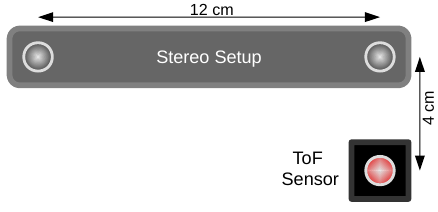
\includegraphics[width=0.5\columnwidth]{tof_stereo_acquisition_system}
    \caption[Sistema di acquisizione ToF-Stereo]{Rappresentazione del sistema di acquisizione ToF-Stereo. Il sensore ToF è posizionato sotto la telecamera di riferimento della coppia stereo.}
    \label{sistema_di_acquisizione}
\end{figure}

\subsection{Sistema di visione stereo}
Il sensore a visione stereoscopica consiste nell'acquisire due immagini bidimensionali da una coppia di telecamere rettificate, ossia allineate lungo un asse che inquadrano la stessa scena. Lo stesso punto P dello spazio viene proiettato nel piano dell'immagine di ciascuna delle telecamere. I punti risultanti \(p_L\) e \(p_R\), detti \textit{omologhi}, hanno le stesse coordinate verticali, considerata la rettificazione dei sensori. Viene chiamata \textit{disparità} lo scostamento tra le coordinate orizzontali: \[d = u_L - u_R\] Tramite questo valore è possibile determinare la posizione del punto P nello spazio.\\
Uno dei principali vantaggi è il costo ridotto delle telecamere CCD o CMOS, facilmente accessibili nel mercato. Tale sensore è inoltre passivo, quindi può sfruttare l’illuminazione dell’ambiente. Ciò permette di essere utilizzato in ambienti esterni, al contrario di altri sensori che sfruttano
pattern proiettati con illuminatori. Inoltre può avere alte risoluzioni e una limitata quantità di rumore.\\
Lo svantaggio maggiore è la dipendenza dei risultati forniti da questi sensori dalla tessitura delle immagini utilizzata nel calcolo degli omologhi, ad esempio sono evidenti delle difficoltà nell'analisi di scene con pattern uniformi o ripetitivi. Pertanto essi presentano un’accuratezza solitamente limitata.

\begin{figure}[ht]
    \centering
    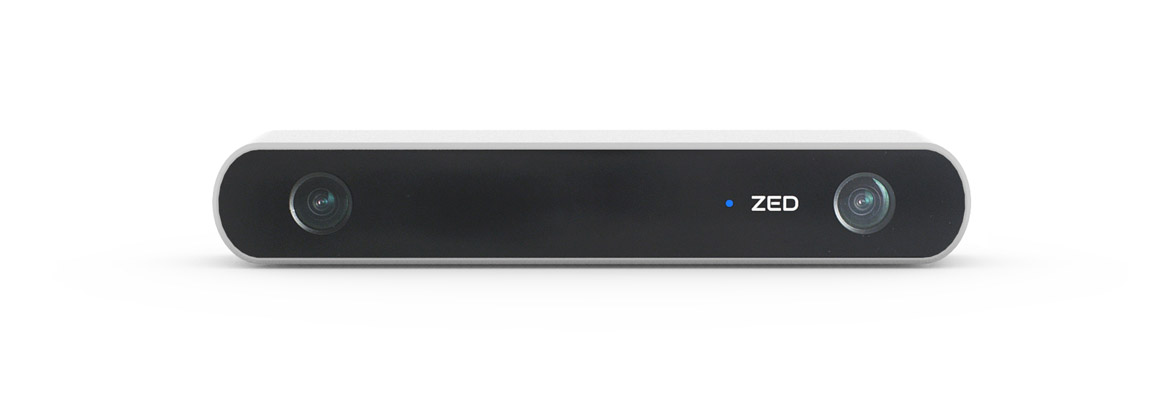
\includegraphics[width=0.5\columnwidth]{ZED}
    \caption[Sensore di visione stereo]{Sensore stereo ZED}
    \label{zed}
\end{figure}

\subsection{Sensore Time-Of-Flight}
Il sensore ToF determina le informazioni riguardo la profondità sulla base del fatto che le onde elettromagnetiche viaggiano alla velocità \(c\approx3\times 10^8[m/s]\). Il sensore emette un impulso luminoso (tipicamente infrarosso) il quale colpisce la scena e viene riflesso indietro. Viene dunque misurato il tempo $\tau$ che occorre al segnale luminoso per percorrere un tragitto pari al doppio della distanza dell'oggetto dalla telecamera $\rho$. La relazione che lega $\rho$ e $\tau$ è $$\rho=\frac{c\tau}{2}$$
Per misurare il tempo cercato e migliorare la risoluzione del sensore, l'impulso emesso è modulato secondo un segnale sinusoidale, così che anche l'eco abbia lo stesso andamento, ma
sfasato e attenuato in ampiezza.
\begin{figure}[ht]
    \centering
    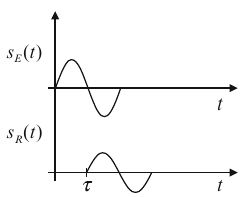
\includegraphics[width=0.4\columnwidth]{time-of-flight}
    \caption[Principio time-of-flight]{Segnale sinusoidale trasmesso e corrispondente segnale ricevuto da un sensore ToF}
    \label{tof}
\end{figure}\\
Dispositivi ToF costituiti da un singolo trasmettitore e un singolo ricevitore, vengono tipicamente utilizzati in telemetri laser. Al fine di realizzare una mappa bidimensionale dell'ambiente, un sistema è quello di montare il sensore su una piattaforma roteante, tale configurazione ha trovato l'utilizzo nel campo dell'automobilistica. Il sistema utilizzato in questo lavoro di tesi appartiene bensì alla famiglia dei sensori ToF scanner-less chiamati anche ToF camera.
\paragraph{ToF camera}
Nelle ToF camera, gli impulsi luminosi sono segnali infrarossi inviati tramite LED e il ricevitore è una matrice di sensori CCD/CMOS. Diversamente dal meccanismo di tipo scanner, le ToF camera catturano le geometrie della scena in un singolo scatto nella quale ogni pixel misura, indipendentemente dalle altre, la distanza del punto della scena di fronte.
\begin{figure}[ht]
    \centering
    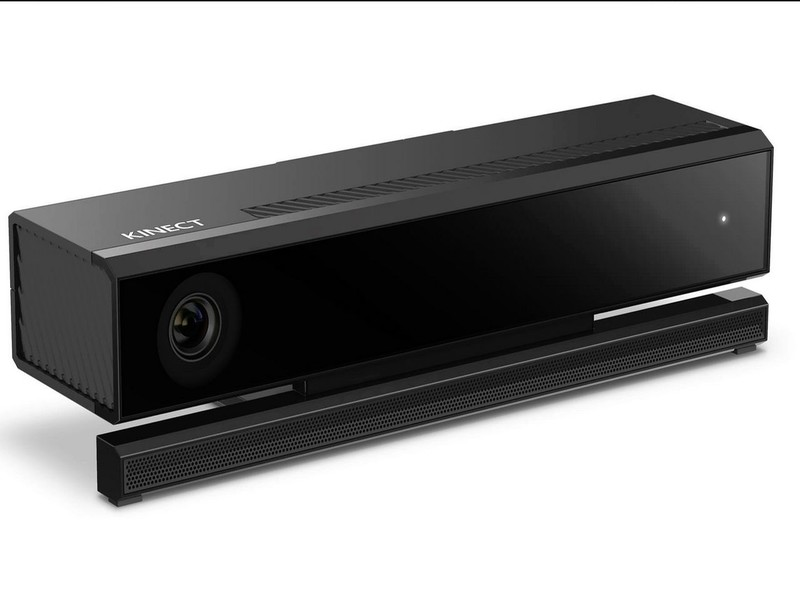
\includegraphics[width=0.3\columnwidth]{kinect}
    \caption[Microsoft kinect]{Il Microsoft Kinect è un esempio di ToF Camera}
    \label{zed}
\end{figure}\\
I vantaggi maggiori sono, al contrario delle telecamere stereo, l'indipendenza dal contenuto della scena, e la maggiore rapidità poichè non richiede algoritmi particolari per il calcolo della disparità. \\
Tuttavia, la tecnologia non è esente da alcune limitazioni: 
\begin{itemize}
    \item Per superfici poco riflettenti o di colore scuro, il segnale di ritorno è debole, ciò risulta in misure poco accurate. 
    \item La limitata risoluzione spaziale non permette di ricavare una informazione dettagliata della geometria della scena.
    \item Il "multipath error" è un ulteriore problema che appare tipicamente vicino alle zone di incidenza tra le superfici. Esso è provocato dalla riflessione multipla del segnale luminoso prima di raggiungere il sensore. 
\end{itemize}

\section{Il Machine Learning}
Il machine learning, o apprendimento automatico, è una branca dell'informatica che fornisce ai computer la capacità di imparare ad eseguire un task da una certa esperienza, senza essere esplicitamente programmati a farlo. In sostanza, il machine learning esplora l'utilizzo di metodi matematico-computazionali per apprendere informazioni direttamente dai dati, senza modelli matematici ed equazioni predeterminate. Gli algoritmi di apprendimento automatico migliorano le loro prestazioni in modo "adattivo" mano a mano che gli "esempi" da cui apprendere aumentano. \\
I problemi che il machine learning punta a risolvere vengono classificati in tre categorie:
\begin{itemize}
    \item \textbf{Apprendimento supervisionato}: ogni istanza del set di esempi (training set) presenta gli input e i corrispondenti valori attesi in output. Questi esempi vengono presentati uno per volta alla macchina, il quale deve essere in grado di approssimare l'esatta natura della relazione presente tra l'input e il corrispondente output. L’obiettivo finale è dunque quello di insegnare al modello la capacità di predire correttamente i valori attesi su un set di istanze non presenti nel training set (test set). Questo scenario è quello trattato in questo lavoro di tesi.
    \item \textbf{Apprendimento non supervisionato}: al contrario dell'apprendimento supervisionato, gli output corrispondenti agli input forniti non sono conosciuti. All'algoritmo viene presentato bensì numerosi dati dai quali la macchina deve estrarre le caratteristiche o i pattern nascosti. 
    \item \textbf{Apprendimento per rinforzo}: si basa sul presupposto di potere ricevere degli stimoli dall'esterno a seconda delle scelte dell'algoritmo. Contrariamente all’apprendimento supervisionato nella quale si conosce l’uscita corretta che il sistema deve dare, l’apprendimento per rinforzo viene adoperato quando si ha a disposizione solamente di un’informazione qualitativa (giusto/sbagliato, successo/fallimento), chiamata segnale di rinforzo.
\end{itemize}
Esistono svariati approcci per la progettazione di sistemi di machine learning che vanno dagli alberi di decisione agli algoritmi genetici. La tecnica di interesse per il lavoro di questa tesi è quello basato sulle reti neurali artificiali.

\subsection{Reti neurali artificiali}
Le reti neurali artificiali (in inglese \textit{artificial neural network}, ANN) sono una classe di modelli matematici oggetti di numerosi studi. La loro importanza è derivato dal loro largo utilizzo in differenti ambiti e applicazioni. Da come suggerisce la parte "neurale" del nome, essi sono modelli che ricalcano il complesso funzionamento del sistema nervoso biologico. Le ANN sono composte da unità, chiamati neuroni, e le connessioni tra essi imitano il ruolo delle sinapsi.
\begin{figure}[ht]
    \centering
    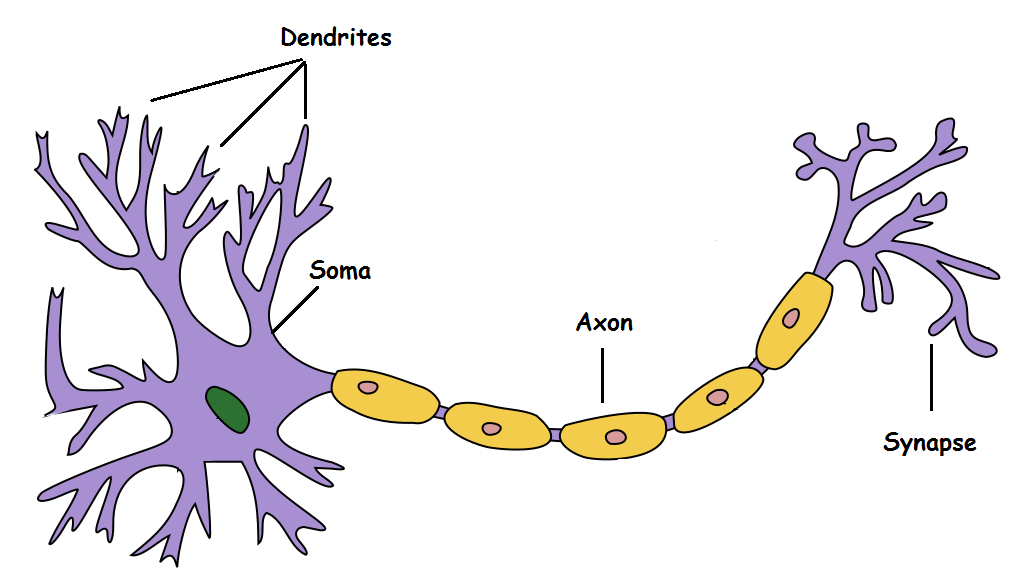
\includegraphics[width=0.5\columnwidth]{biological_neuron}
    \caption[Neurone biologico]{Neurone biologico}
    \label{biological_neuron}
\end{figure}
\paragraph{Percettrone}
Il più semplice modello dei neuroni artificiali è il \textit{percettrone}. 
\begin{figure}[ht]
    \centering
    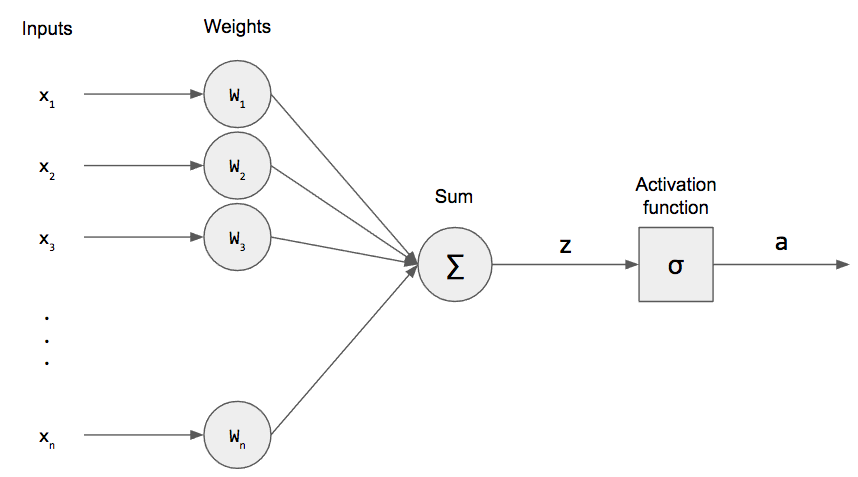
\includegraphics[width=0.5\columnwidth]{perceptron}
    \caption[Percettrone]{Schema di un percettrone}
    \label{biological_neuron}
\end{figure}
Esso prende in input un vettore di valori reali e ne effettua una combinazione lineare, il risultato viene infine passato ad una funzione, detta funzione di attivazione, che restituisce l'output del neurone. Il modello complessivo può essere descritto dalla seguente formula: 
$$y=\sigma(\sum_{i} w_{i}x_{i}+b)$$
dove $w_{i}$ sono i pesi e b è un termine, detto bias, che viene aggiunto in seguito. Nel percettrone classico la funzione di attivazione $\sigma$ è una funzione a gradino, tuttavia sono numerose le alternative: tra i più comuni sono il sigmoide e il rettificatore.
\paragraph{Deep Neural Network} 
Le reti neurali artificiali sono tipicamente organizzati in più strati, i nodi che la compongono sono suddivisi in tre macro-categorie. Abbiamo i nodi appartenenti allo strato di ingresso (input), i nodi appartenenti allo strato di uscita (output) e infine i nodi degli strati nascosti (hidden). L’architettura per strati è tipica delle reti neurali feed-forward. Tali reti sono caratterizzate dal fatto che l’attivazione dei nodi d’ingresso si propaga in avanti verso quelli dello strato (o degli strati) nascosto e da questi verso quelli dello strato di uscita.
\begin{figure}[ht]
    \centering
    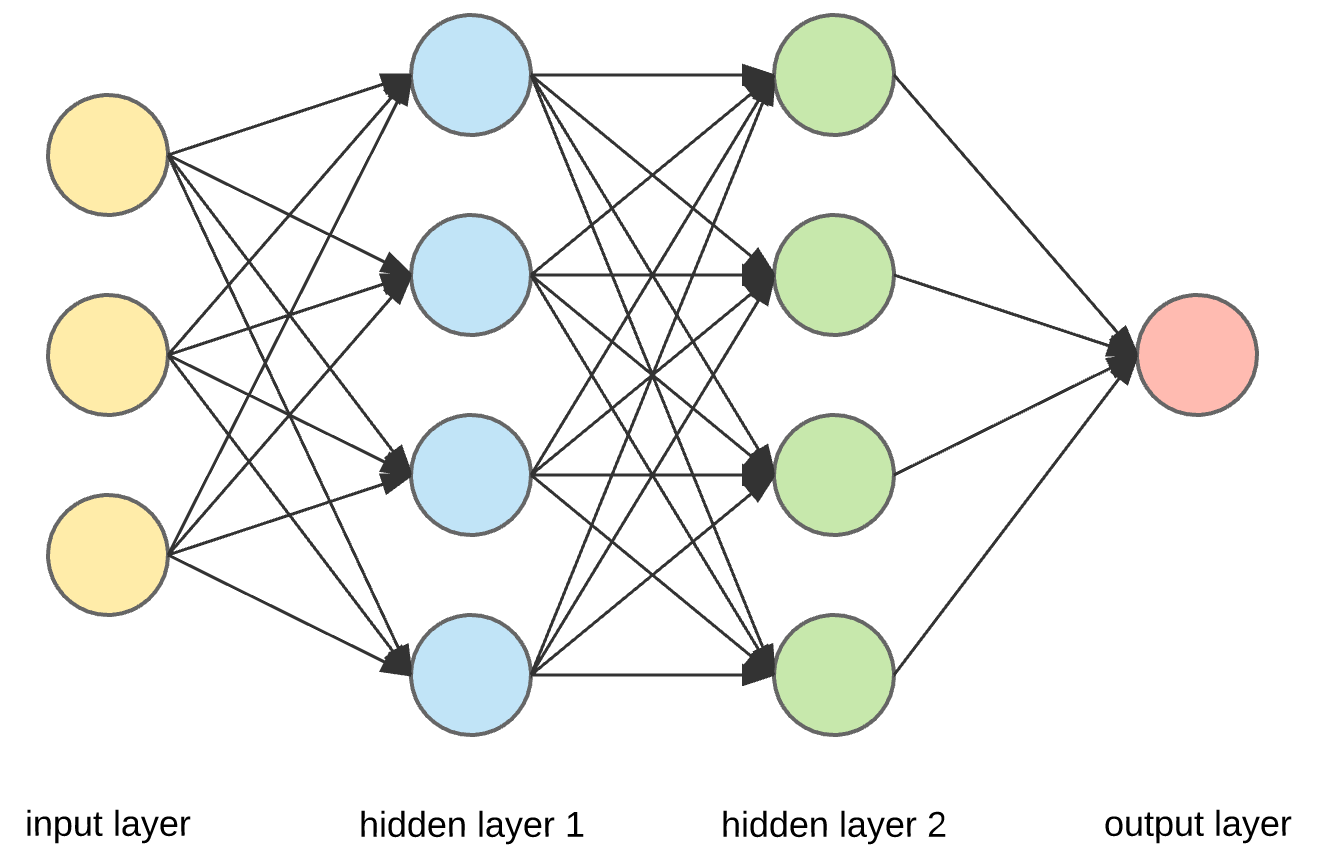
\includegraphics[width=0.5\columnwidth]{DNN}
    \caption[Deep Neural Network]{Rappresentazione di una rete neurale profonda}
    \label{DNN}
\end{figure}

\subsection{Reti neurali convoluzionali}
Le reti neurali visti fino ad ora sono composti da neuroni completamente interconnessi con ogni neurone del precedente e successivo strato. Ciò comporta un numero sproporzionato di pesi che devono essere gestiti all'aumentare degli strati e dei neuroni. Il problema diventa significativo dal punto di vista della memoria e del tempo di addestramento. Un altro svantaggio è l'\textit{overfitting}. Infatti, avere un grosso numero di parametri, implica che se il training set non è abbastanza grosso, la rete potrebbe imparare a discriminare perfettamente gli esempi del training set, però avere scarse prestazioni su dati nuovi.\\
Questi problemi sono stati affrontati efficacemente con le reti neurali convoluzionali (\textit{convolutional neural network}, CNN). Differentemente dalle tradizionali reti neurali, qui i neuroni sono connessi soltanto ad un sottoinsieme dei neuroni dello strato precedente, questa regione viene definita campo recettivo (\textit{receptive field}). Questo modello si ispira alla struttura della corteccia visiva del mondo animale. Nelle CNN approssimiamo la risposta di un singolo neurone agli stimoli del proprio campo recettivo attraverso una operazione di convoluzione.
\paragraph{Convoluzione} 
La convoluzione viene effettuata tra l'input di uno strato e uno o più filtri, detti anche \textit{kernel}. L'output della operazione di convoluzione è detta \textit{feature map}. Ci sono tante feature map quanti sono il numero di filtri utilizzati per elaborare gli input. 
\begin{figure}[ht]
    \centering
    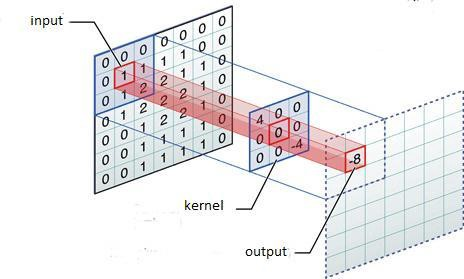
\includegraphics[width=0.5\columnwidth]{convolution}
    \caption[Esempio di convoluzione]{illustrazione della operazione di convoluzione con un filtro}
    \label{convolution}
\end{figure}\\
Il principio di convoluzione è fondamentale: oltre a mantenere limitato il numero di parametri, esso fornisce una proprietà di invarianza alla traslazione. Di fatto, lo stesso filtro viene applicato su tutta l'immagine, ciò permette di rilevare una particolarità nell'immagine ovunque essa sia, indipendentemente dalla sua posizione. 
\paragraph{Funzioni di attivazione}
Analogamente alle reti neurali tradizionali, anche nelle CNN vengono usate le funzioni di attivazione. Questi vengono solitamente messi immediatamente dopo gli strati di convoluzione e hanno lo scopo di permettere alla rete l'apprendimento di funzioni non lineari. 
\begin{figure}[ht]
    \centering
    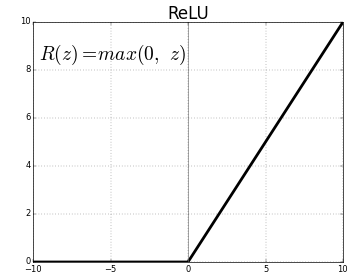
\includegraphics[width=0.3\columnwidth]{relu}
    \caption[Funzione di attivazione relu]{funzione di attivazione ReLU}
    \label{relu}
\end{figure}
La funzione di attivazione più utilizzata in questo campo negli ultimi anni è il rettificatore lineare (\textit{Rectified Linear Unit}, ReLU). Questa, rispetto ad altre funzioni come la tangente iperbolica o la sigmoide, porta ad un processo di allenamento più rapido.
\chapter{Acquisizione e pre-elaborazione dei dati}

\section{Preparazione dei dati ToF}

\subsection{Riproiezione e interpolazione}

\subsection{Calcolo della disparità}

\section{Elaborazione dei dati stereo}

\subsection{Disparità stereo}
\chapter{Fusione tramite deep learning}

\section{Le componenti della CNN}
\subsection{Reti neurali residuali}
Le reti neurali residuali, o ResNet, sono stati introdotti da Microsoft nel 2015 battendo il record della competizione ILSVRC con un errore del 3.6\% \cite{resnet}, superando per la prima volta le prestazioni umane.\\
L'idea che sta alla base delle reti neurali residuali è l'utilizzo di un particolare tipo di blocco, il \textit{residual block}, che sfrutta il concetto delle \textit{skip connection}. \\
Vediamo ora il modello del residual block:
\begin{figure}[ht]
    \centering
    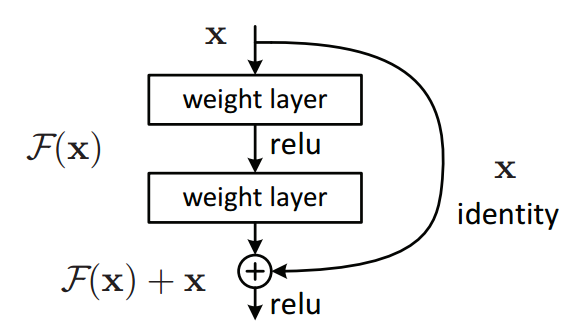
\includegraphics[width=0.5\columnwidth]{res_block.png}
    \caption[Residual block]{Schema del residual block}
\end{figure}\\
Ogni blocco consiste in una serie di strati, ottenendo una certa $F(x)$, seguito da una \textit{skip connection} che aggiunge al risultato l'input del blocco stesso. Dunque in uscita dal blocco si ha
$$ H(x)=F(x)+x $$
Attraverso la concatenazione di blocchi di questo tipo, ResNet impara a predire l'output non attraverso l'apprendimento di una trasformazione diretta dei dati di input, ma attraverso l'apprendimento del termine $F(x)$, detto \textit{residuo}, da sommare al dato di input per arrivare all'output. Tale modello semplifica la costruzione di strati di identità, basta infatti spingere $F(x)$ verso zero e lasciare l'output come x. Ciò permette agli strati più profondi della rete di alterare poco i concetti già appresi dagli strati precedenti, preservando così le informazioni. Questa architettura ha permesso di creare reti molto più profonde, fino a 152 strati.

\subsection{Batch Normalization}
Durante il processo di addestramento, gli esempi del training set vengono processati in gruppi, detti mini-batch, di dimensione fissa per velocizzare la fase di train sfruttando il parallelismo offerto dalle GPU. La \textit{Batch Normalization} è una tecnica che consiste nel normalizzare i dati del mini-batch ad ogni strato intermedio della rete. In questo modo si riduce il così detto \textit{Internal Covariance Shift}. L'utilizzo del batch normalization ha l'intento di velocizzare il training della rete neurale e migliorarne la stabilità e le performance. Questa operazione si è rivelata particolarmente efficace nelle reti neurali residuali.

\subsection{Bottleneck}
Il modello ResNet introduce il così detto design a "collo di bottiglia". L'idea che sta dietro all'utilizzo di questo design è quello di ridurre le dimensioni dell'input del blocco residuale prima di effettuare la convoluzione 3x3.
\begin{figure}[ht]
    \centering
    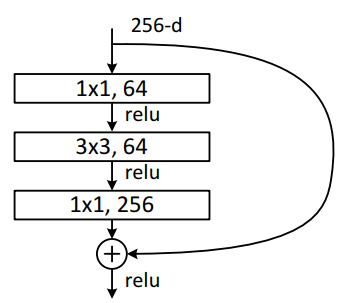
\includegraphics[width=0.4\columnwidth]{bottleneck.png}
    \caption[Bottleneck]{Il design a collo di bottiglia utilizzato dal  ResNet}
\end{figure}
La riduzione della dimensionalità viene eseguita con uno strato di convoluzione 1x1, lasciando lo strato di convoluzione 3x3 con delle dimensioni di input/output più ridotte, tenendo così un numero di parametri molto più ristretto. Infine, l'ultimo strato 1x1 ha lo scopo di ripristinare le dimensioni a quelle iniziali. Questo permette un tempo di addestramento più veloce, senza pesare sulle prestazioni \cite{resnet}.

\subsection{Convoluzione dilatata}
Il vantaggio della convoluzione dilatata è la possibilità di catturare più indizi dall'input, espandendo il campo recettivo di una convoluzione 2D.
\begin{figure}[ht]
    \centering
    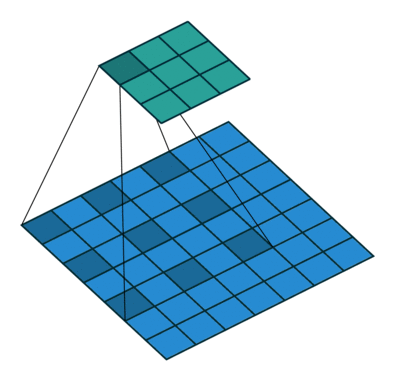
\includegraphics[width=0.5\columnwidth]{dilated_convolution.png}
    \caption[Convoluzione dilatata]{Illustrazione della convoluzione dilatata}
\end{figure}\\
In realtà, anche utilizzando un filtro di dimensioni maggiori si ha un receptive field allargato, ad esempio una convoluzione 3x3 dilatata con rate $r=2$ ha lo stesso campo recettivo di una normale convoluzione 5x5. Tuttavia, il numero di parametri del modello con dilatazione può essere notevolmente ridotto. Un kernel $k\times k$ mantiene, infatti, $k\times k$ parametri avendo però un campo recettivo pari a $k_e\times k_e$ con $k_e=k+(k-1)(r-1)$.

\section{la rete neurale selezionata}
L'architettura della rete neurale convoluzionale utilizzata in questo lavoro di tesi è formato da una rete neurale residuale con bottleneck, batch normalization e convoluzione dilatata. Il blocco residuale utilizzato è il seguente:
\begin{figure}[ht]
    \centering
    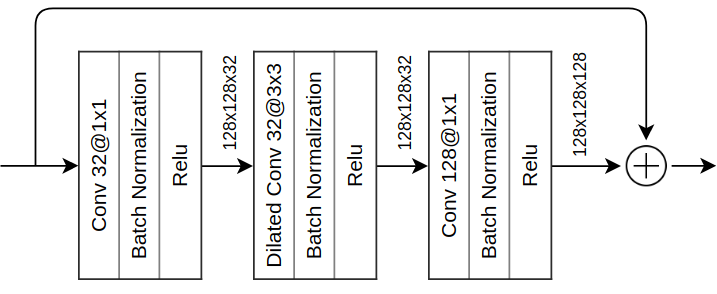
\includegraphics[width=0.6\columnwidth]{my_res_block.png}
    \caption[Diagramma del blocco residuale]{Diagramma del blocco residuale}
\end{figure}

\section{Il processo di training}
\subsection{Loss function e ottimizzazione}
\paragraph{Loss function} Per poter minimizzare l'errore di output della rete neurale è necessario definire tale errore.\\
Le due funzioni di loss valutate in questo lavoro sono le norme l1 e l2, detti anche \textit{mean absolute error} e \textit{mean squared error}.
$$MAE=\frac{1}{n} \sum_{j=1}^{n} |y_j-\hat{y_j}|$$
$$MSE=\frac{1}{n} \sum_{j=1}^{n} (y_j-\hat{y_j})^2$$
Da un veloce confronto, le due norme danno simili risultati sperimentali. È stato deciso di utilizzare la norma l2 che si tratta anche della loss function maggiormente utilizzata.

\subsection{Inizializzazione delle variabili}
\subsection{Iperparametri}
batch size e learning rate
\subsection{Early stopping}

\chapter{Analisi dei risultati}

\section{Framework e ambiente di lavoro}
Per la generazione del dataset a partire dai dati acquisiti è stato utilizzato l'ambiente MATLAB, nel quale sono state anche fatte le operazioni di data augmentation come ritaglio, ribaltazione e rotazione. Mentre per lo sviluppo del modello sono state utilizzate le API Keras su backend TensorFlow in linguaggio di programmazione Python.\\
L'ambiente sul quale è stato eseguito il training è quello fornito da Google Colaboratory in cloud ossia un sistema con Ubuntu 18.04 e scheda grafica Tesla K80.

\section{Training e validation}
Con l'architettura presentata e una volta pronto il codice necessario, è stato possibile procedere con il training della rete e con la successiva valutazione dei risultati.
Gli iperparametri dell'addestramento sono stati impostati nel seguente modo:
\begin{itemize}
    \item durata del training: 75 epoche
    \item learning rate: 0.001
    \item batch size: 32, il più alto possibile con la memoria GPU a disposizione.
    \item loss function: MSE
\end{itemize}
Il tempo per completare il training è stato di circa 1 ora e 40 minuti.\\
In figura \ref{training} e \ref{validation} sono mostrati i grafici degli andamenti del loss di training e validation.
\begin{figure}[H]
    \centering
    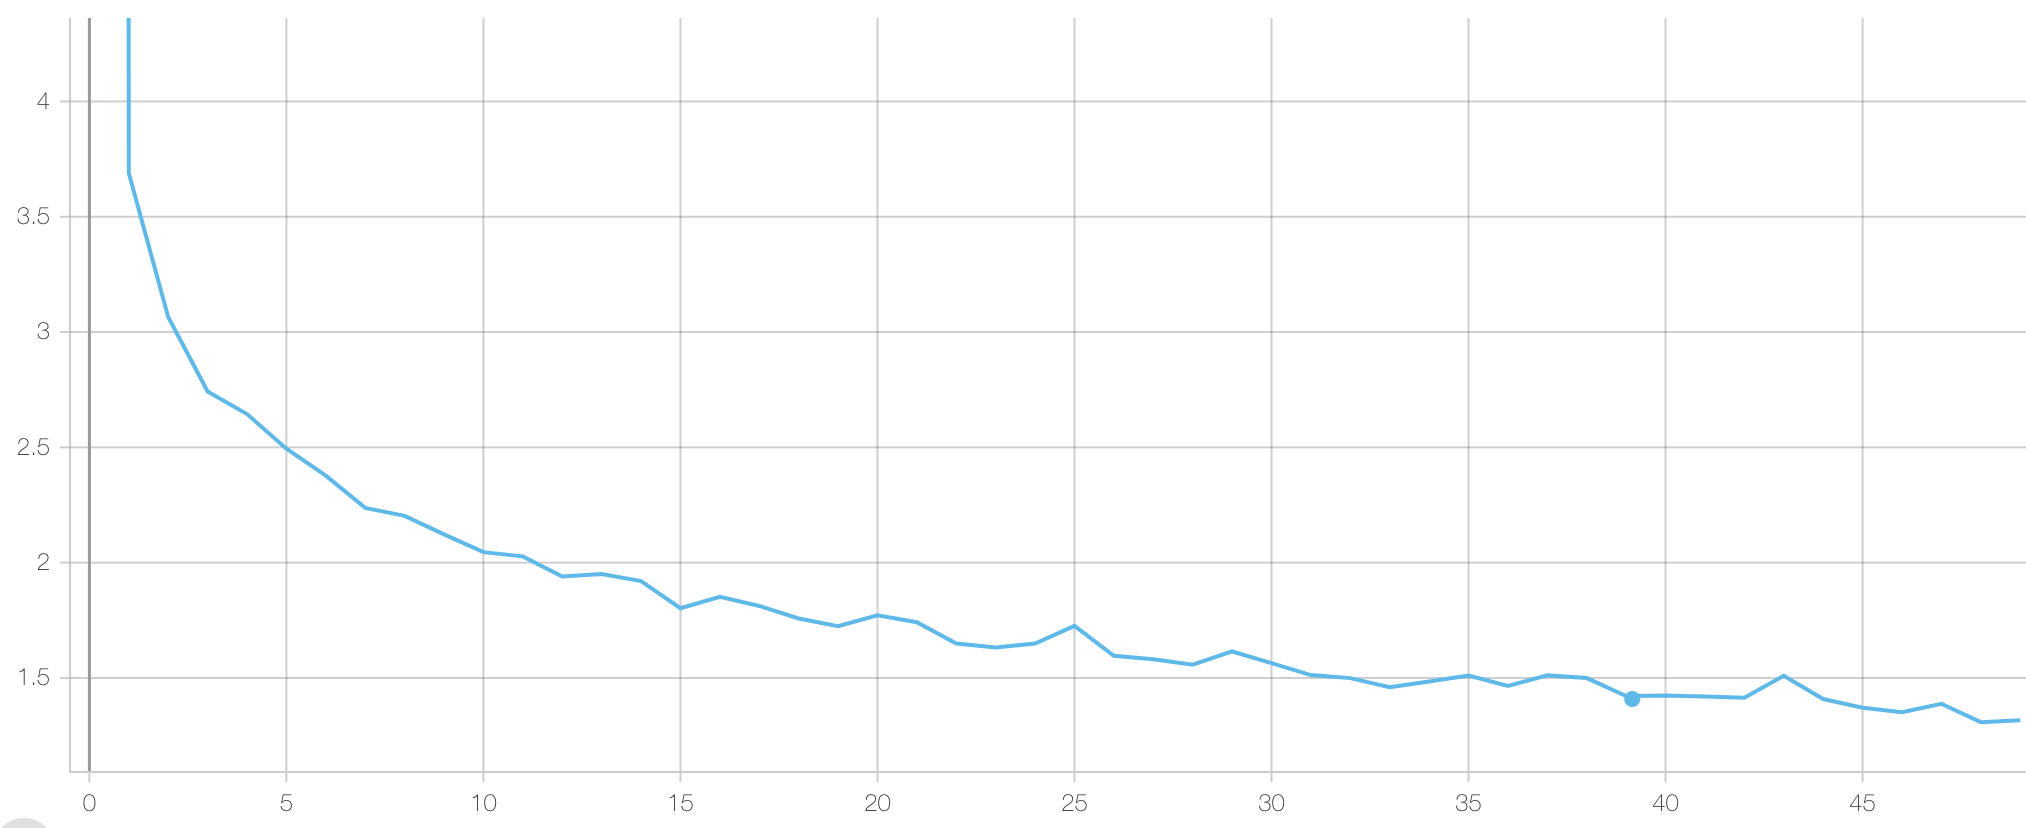
\includegraphics[width=1.0\columnwidth]{final_training.png}
    \caption[Andamento del training loss]{Andamento del training loss}
    \label{training}
\end{figure}

\begin{figure}[H]
    \centering
    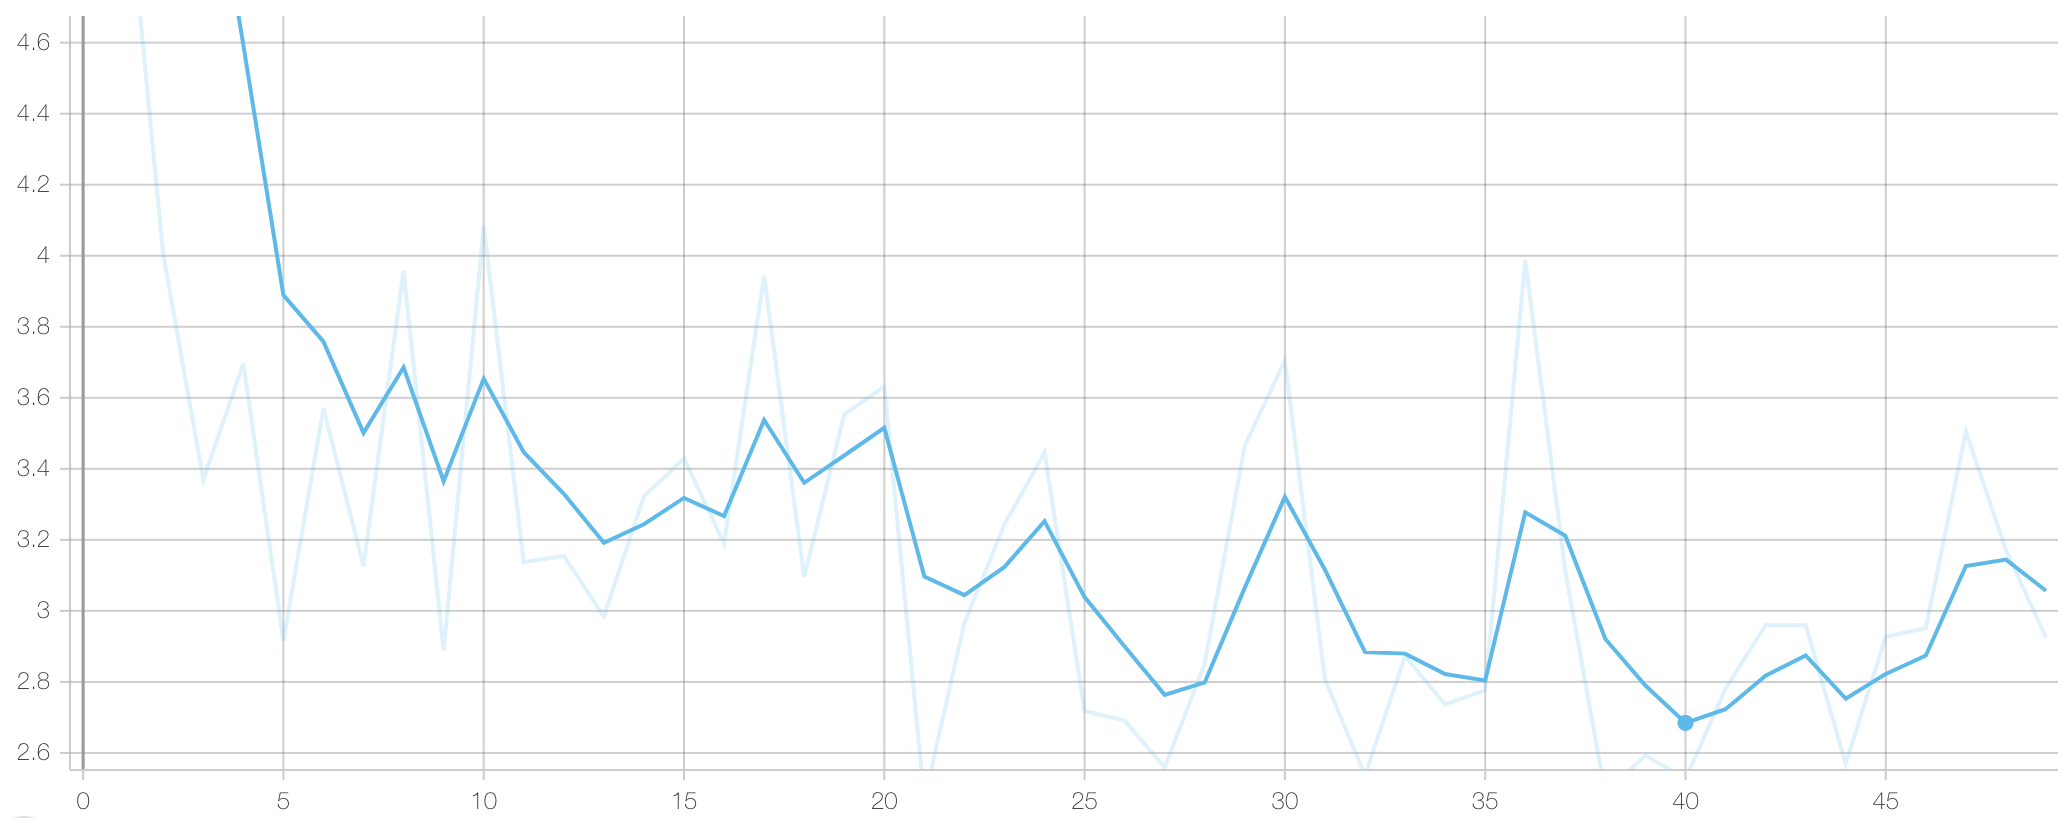
\includegraphics[width=1.0\columnwidth]{final_validation.png}
    \caption[Andamento del validation loss]{Andamento del validation loss}
    \label{validation}
\end{figure}

\section{Test e risultati sperimentali}
Nelle figure seguenti sono mostrati alcuni risultati sperimentali della rete addestrata. La prima e la seconda colonna mostrano gli input ToF e Stereo rispettivamente. Si nota nei dati ToF la presenza di alcuni "buchi" sulle superfici poco riflettenti e sulle regioni affette dal "multipath error", ossia in prossimità delle zone di incidenza tra le superfici. Per quanto riguarda lo stereo, si notano in particolare accuratezze limitate sui bordi.\\
La terza colonna mostra la fusione, ossia l'output della rete. Infine nella quarta colonna vengono illustrati i ground truth. La fusione è in grado di estrarre le informazioni più accurate da entrambe le sorgenti, tappando le lacune del ToF ed eliminando gli artefatti lungo i bordi dello stereo.\\
\begin{minipage}{\textwidth}
    \noindent\makebox[\linewidth][s]{\textbf{ | ToF Input | Stereo Input | Output Disparity | Ground Truth |}}\\
    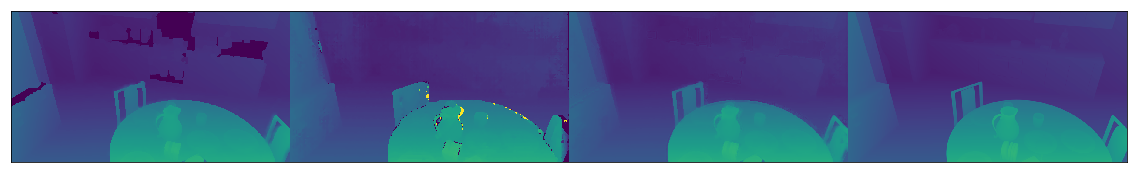
\includegraphics[width=1.0\columnwidth]{test_fig_1.png}
    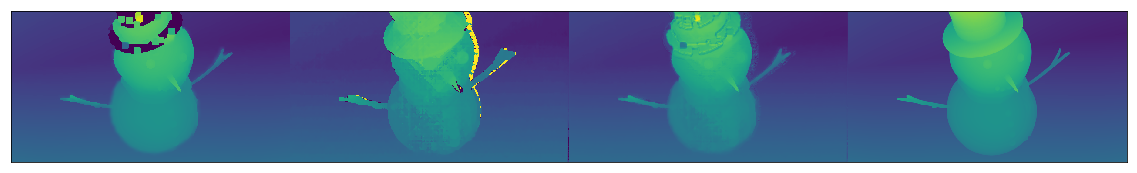
\includegraphics[width=1.0\columnwidth]{test_fig_2.png}
    
\includegraphics[width=1.0\columnwidth]{test_fig_3.png}
    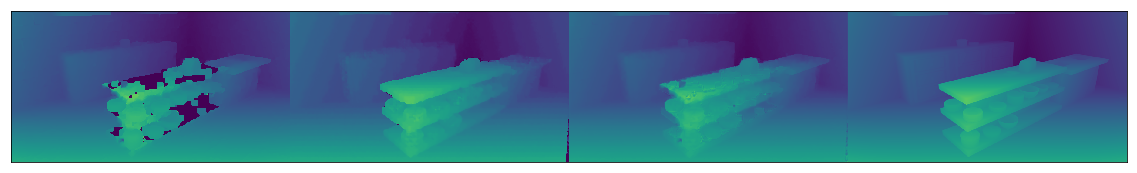
\includegraphics[width=1.0\columnwidth]{test_fig_4.png}
\end{minipage}

\section{Confronti tra differenti architetture}
\paragraph{La nostra rete contro una rete elementare}Confrontiamo ora i risultati che abbiamo ottenuto contro quelli acquisiti da una semplice rete illustrata in figura \ref{simple_net}. Questa architettura non include blocchi residuali, normalizzazioni e convoluzioni dilatate.
\begin{figure}[ht]
    \centering
    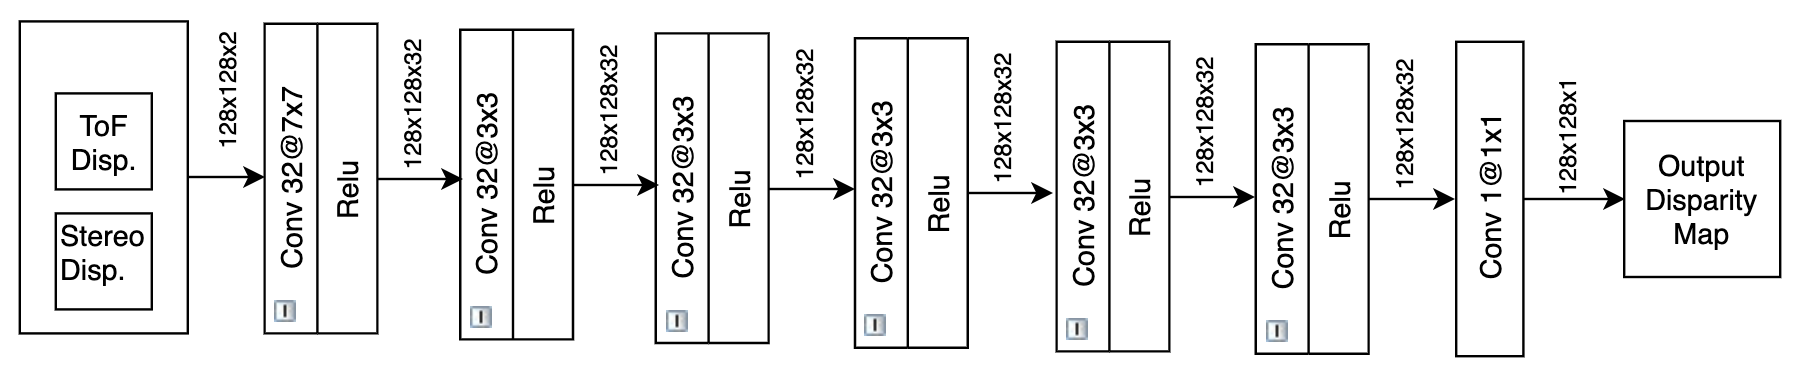
\includegraphics[width=1.0\columnwidth]{simple_net.png}
    \caption{Diagramma di una semplice CNN senza blocchi residuali, convoluzioni dilatate e normalizzazioni}
    \label{simple_net}
\end{figure}

\begin{figure}[ht]
    \centering
    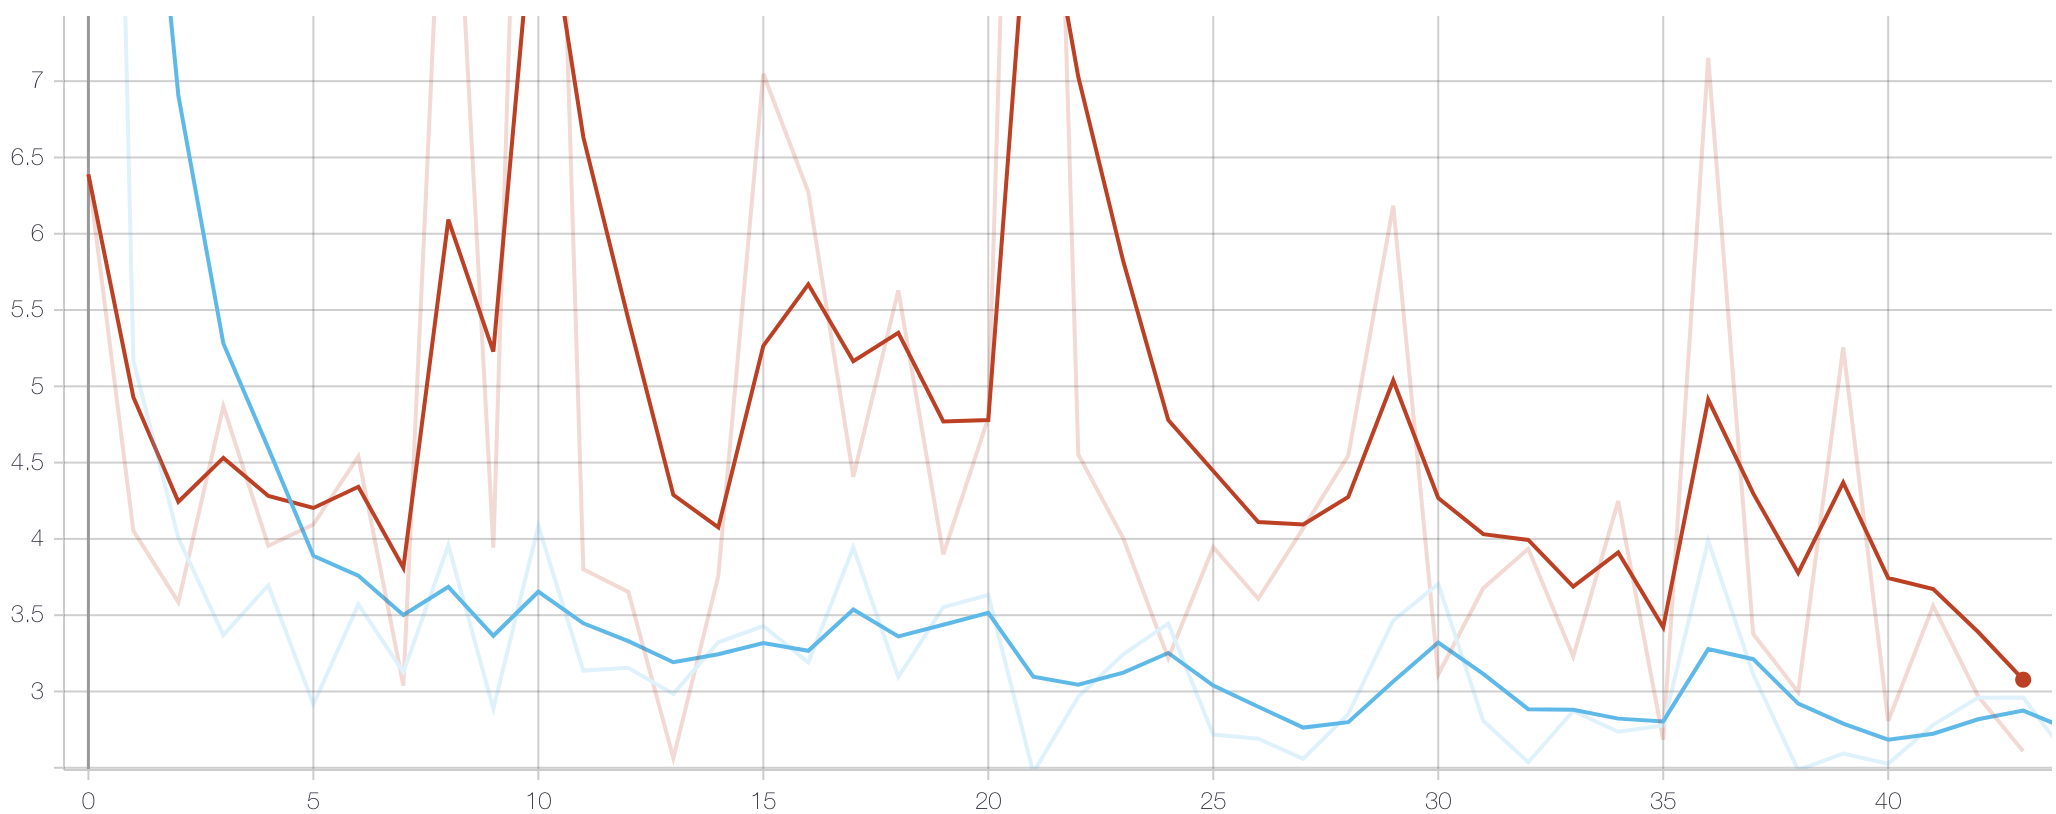
\includegraphics[width=0.8\columnwidth]{simplenet_vs_final.png}
    \caption[Confronto del validation loss di DRFNet contro una versione più elementare]{
        Confronto del validation loss di DRFNet contro una versione più elementare. \\
        \definecolor{final}{RGB}{187,187,187}
        \definecolor{elementar}{RGB}{238,120,80}
        \fcolorbox{black}{final}{\rule{0pt}{6pt}\rule{6pt}{0pt}}\quad DRFNet (figura \ref{my_net})\\
        \fcolorbox{black}{elementar}{\rule{0pt}{6pt}\rule{6pt}{0pt}}\quad La CNN elementare (figura \ref{simple_net})
    }
    \label{simplevsfinal}
\end{figure}

Si nota immediatamente dalla figura \ref{simplevsfinal} che la nostra rete performa assai meglio della rete con architettura elementare convergendo molto più rapidamente e con meno oscillazioni.

\paragraph{Convoluzione dilatata contro senza dilatazione} Proviamo ora a togliere la dilatazione dagli strati di convoluzione della nostra rete. Proviamo quindi a comparare i risultati così ottenuti con quelli acquisiti con la dilatazione.
\begin{figure}[H]
    \centering
    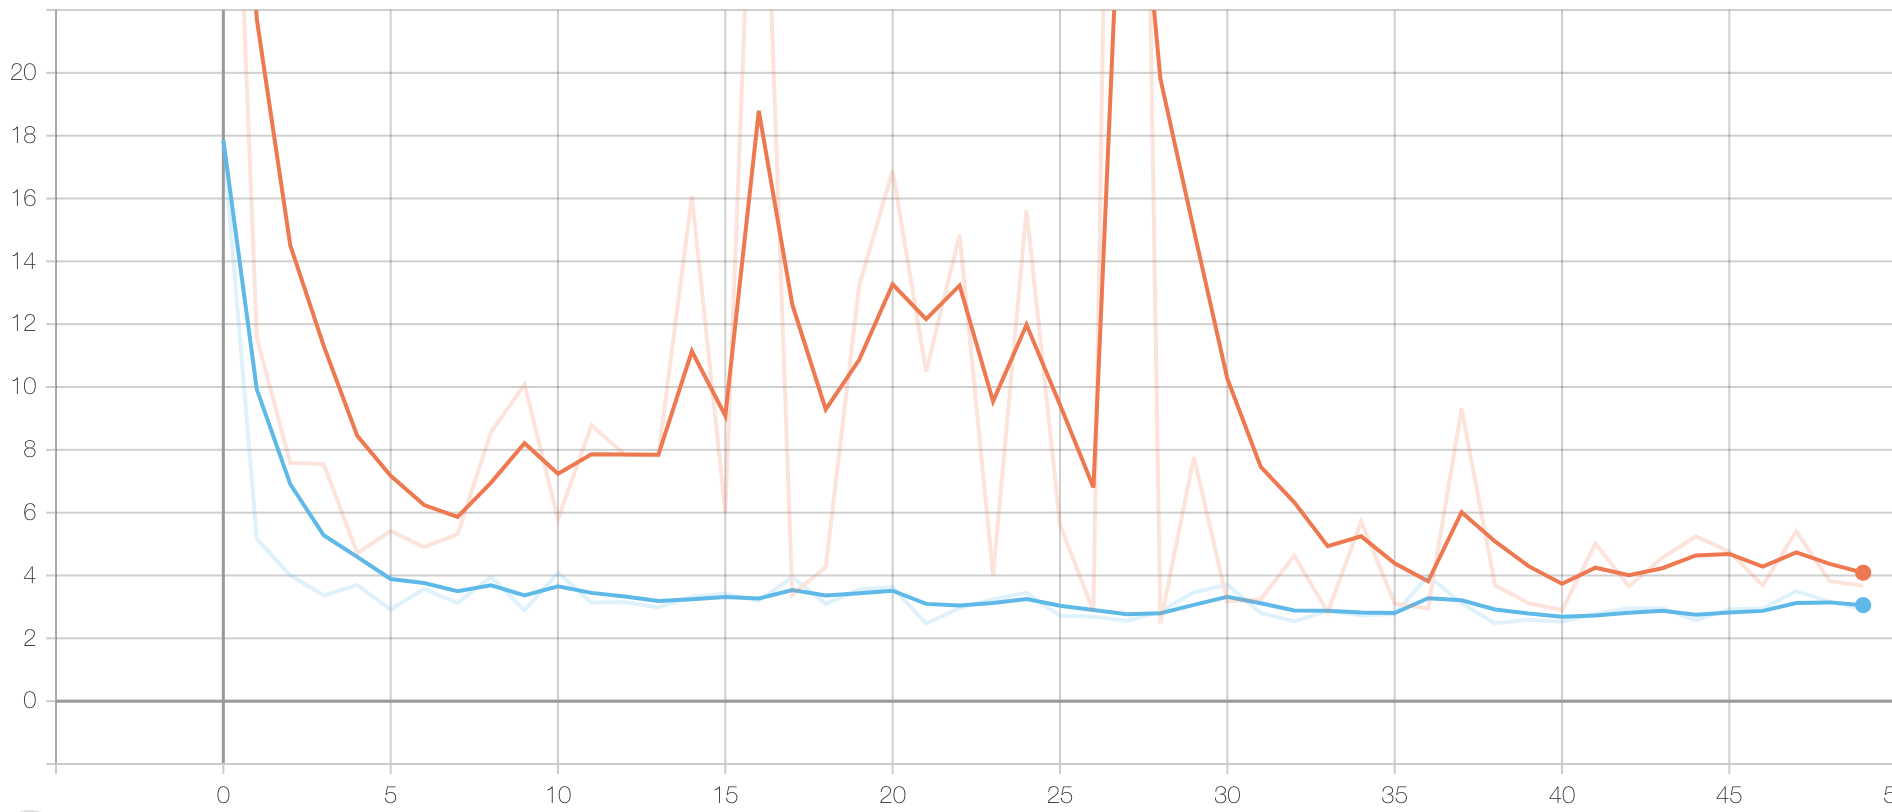
\includegraphics[width=0.8\columnwidth]{dilation_vs_nodilation.png}
    \caption[Confronto del validation loss della rete con strati di convoluzione dilatata contro senza dilatazione]{
        Confronto del validation loss della rete con strati di convoluzione dilatata contro senza dilatazione. \\
        \fcolorbox{black}{cyan}{\rule{0pt}{6pt}\rule{6pt}{0pt}}\quad DRFNet (figura \ref{my_net})\\
        \fcolorbox{black}{orange}{\rule{0pt}{6pt}\rule{6pt}{0pt}}\quad La rete senza dilatazione sulla convoluzione
    }
    \label{dilation_vs_nodilation}
\end{figure}
Come si vede dalla figura \ref{dilation_vs_nodilation}, la dilatazione negli strati di convoluzione ha un effetto positivo sulle performance della rete sul validation set. È possibile difatti apprezzare un andamento migliore e più stabile nel caso dell'utilizzo della dilatazione.

\paragraph{Comparazioni tra diverse profondità della rete}
Con l'obiettivo di determinare la migliore profondità della rete, proviamo a variare il numero di blocchi residuali tra 4, 6 e 8. 
\begin{figure}[H]
    \centering
    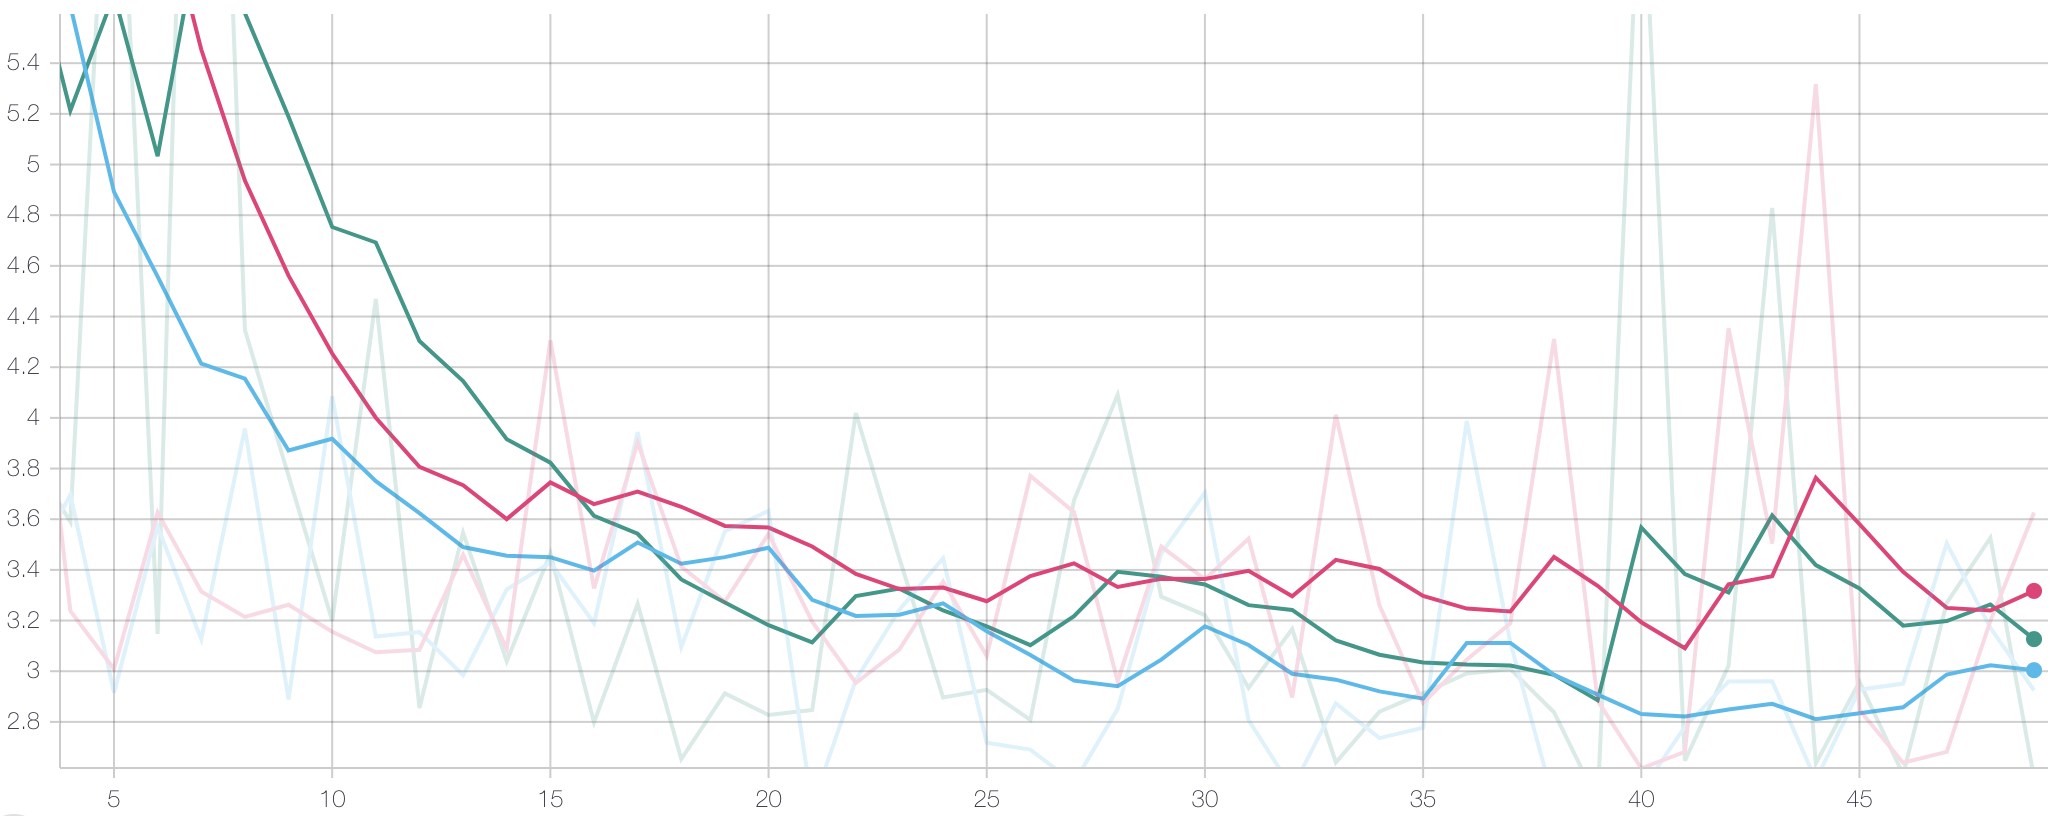
\includegraphics[width=0.8\columnwidth]{depth_compare.png}
    \caption[Confronto tra differenti numeri di blocchi residuali]{
        Confronto tra differenti numeri di blocchi residuali. \\
        \fcolorbox{black}{cyan}{\rule{0pt}{6pt}\rule{6pt}{0pt}}\quad 6 blocchi residuali\\
        \definecolor{four}{RGB}{219,70,119}
        \definecolor{eight}{RGB}{67,150,176}
        \fcolorbox{black}{four}{\rule{0pt}{6pt}\rule{6pt}{0pt}}\quad 4 blocchi residuali\\
        \fcolorbox{black}{eight}{\rule{0pt}{6pt}\rule{6pt}{0pt}}\quad 8 blocchi residuali
    }
    \label{depth_compare}
\end{figure}
Dal grafico comparativo di figura \ref{depth_compare} si vede un andamento leggermente migliore nel caso dell'utilizzo di 6 blocchi residuali, con 8 blocchi si hanno risultati molto simili mentre il caso peggiore è quello con 4 blocchi.
\chapter{Conclusioni}
L'obiettivo di questa tesi è stata quella di costruire un sistema in grado di fondere i dati tridimensionali forniti da due diversi tipi di sensori, ossia un sensore a tempo di volo e una coppia di telecamere stereo.\par
I risultati riportati hanno mostrato come l'utilizzo di tecniche di deep learning all'avanguardia, permetta di realizzare un modello in grado di sfruttare al meglio le informazioni fornite dai due sensori, realizzando una ricostruzione più accurata delle strutture tridimensionali della scena catturata. In particolare si è visto come l'utilizzo delle reti neurali residuali assieme alle convoluzioni dilatate abbia effettivamente apportato benefici tangibili sulle performance della rete nella stima della disparità.\par
I risultati ottenuti da questo lavoro di tesi possono inoltre essere applicati per la fusione di una diversa combinazione di sensori al fine di ottenere risultati simili oppure migliori.\par
Possibili sviluppi futuri comprendono sicuramente il test della rete neurale addestrata, su un dataset reale per verificare le performance del modello su dati del mondo reale.


%\appendix

%\input{appendici}

\backmatter

%\addcontentsline{toc}{chapter}{Bibliografia}
\nocite{*}
\bibliographystyle{plain}
\bibliography{tesi}

% si può scegliere di utilizzare direttamente l'imput di un file 'biblio.tex' da editare a mano.
%\input{biblio}

\printindex % se si fa l'indice analitico.

\end{document}

